\documentclass[parskip=full,11pt,twoside]{scrartcl}

\usepackage[sfdefault,light]{roboto}
\usepackage{inconsolata}
\usepackage[ngerman]{babel}

\usepackage[utf8]{inputenc}
\usepackage[T1]{fontenc}

\usepackage{microtype}

\usepackage{csquotes}
\MakeOuterQuote{"}

\usepackage{graphicx}
\usepackage{float}
\usepackage{bm}
\usepackage{amssymb}
\usepackage[hidelinks]{hyperref}
\usepackage[section]{placeins}

\titlehead{\centering
\includegraphics[width=6cm]{img/logo.pdf}}
\title{Implementierungsbericht}
\subtitle{Wavelength--$\bm{\lambda}$-IDE}
\author{Muhammet Guemues, Markus Himmel, Marc Huisinga,\\Philip Klemens, Julia Schmid, Jean-Pierre von der Heydt}

\begin{document}
\maketitle
\newpage
\tableofcontents
\newpage

\section{Einleitung}
Nach einer groben Skizze der Anwendung im Pflichtenheft und einer genaueren Spezifikation in der Entwurfsphase folgt nun eine Vorstellung der konkreten Implementierung.
Die Erfüllung der geforderten Spezifikationen erfordert den Einsatz verschiedener Bibliotheken, die kurz vorgestellt werden sollen:

\subsection{Google Web Toolkit (GWT)}
\begin{enumerate}
\item[] \textbf{Ziel:} Programmierung der Anwendung in Java 
\item[] \textbf{Beschreibung:} Das Google Web Toolkit kompiliert Java-Quellcode zu JavaScript, welches direkt im Webbrowser des Anwenders läuft. Zusätzlich
werden Werkzeuge bereitgestellt, um die Benutzeroberfläche der Webapplikation direkt in Java zu konstruieren.
\item[] \textbf{Erläuterung:} Ziel dieses Projektes ist die Entwicklung einer Online-Ent\-wick\-lungs\-um\-ge\-bung für den untypisierten $\lambda$-Kalkül.
Diese unterliegt der Einschränkung, in einer statisch typisierten Programmiersprache verfasst zu werden (siehe Pflichtenheft unter N4).
Um dieser Anforderung nachzukommen, wird die Anwendung in Java programmiert und mit GWT im Webbrowser ausgeführt.
\end{enumerate}

\subsection{GWT-Bootstrap}
\begin{enumerate}
\item[] \textbf{Ziel:} Optisch ansprechende Benutzeroberfläche 
\item[] \textbf{Beschreibung:} GWT-Bootstrap stellt Java-Klassen für die Verwendung von Bootstrap-Komponenten mit GWT bereit.
\item[] \textbf{Erläuterung:} Für die Entwickler waren die von GWT bereitgestellten GUI-Elemente optisch inkohärent und von niederer Anmut.
Ein stimmigeres Bild fanden sie in den von Bootstrap bereitgestellten Komponenten.
Die Verwendung dieser Komponenten mit GWT erwies sich jedoch als umständlich.
Um diese Komponenten trotzdem verwenden zu können, wurde GWT-Bootstrap eingebunden, das die Verwendung erheblich erleichtert.
Darüber hinaus stellt die Bibliothek auch Icons zur Verfügung, die für die GUI verwendet werden (siehe dazu beispielsweise Pflichtenheft Anhang A).
Der Vorteil dieser Icons ist, dass sie einen Satz bilden, also ein konsistentes Bild bieten.
\end{enumerate}

\subsection{Monaco}
\begin{enumerate}
\item[] \textbf{Ziel:} Bereitstellung eines Editors 
\item[] \textbf{Beschreibung:} Monaco ist ein Code-Editor, der in der Software Visual Studio Code verwendet wird, aber auch als freistehende
Bibliothek zur Verfügung steht.
\item[] \textbf{Erläuterung:} Die Entwicklung eines Editors steht bei diesem Projekt nicht im Fokus.  Daher bietet es sich an, hier auf eine Bibliothek zurückzugreifen.
Darüber hinaus wird der Monaco-Editor nicht nur den gestellten Anforderungen gerecht, sondern bietet viele weitere Features.
\end{enumerate}

\subsection{vis.js}
\begin{enumerate}
\item[] \textbf{Ziel:} Erstellung interaktiver Graphen 
\item[] \textbf{Beschreibung:} Bei vis.js handelt es sich um eine Bibliothek für Visualisierungen aller Art mittels JavaScript.
\item[] \textbf{Erläuterung:} Die Ausgabe von $\lambda$-Termen in Form eines Syntaxbaums gestaltet sich als nicht-triviale Aufgabe.
Dieser muss nicht nur konstruiert werden, sondern auch noch stellenweise klickbar sein (siehe dazu Pflichtenheft unter F5).
Die Modellierung der Daten erfolgt als Java-Quellcode; lediglich die Visualisierung baut auf der JavaScript-Bibliothek auf.
\end{enumerate}

\subsection{SQLite}
\begin{enumerate}
\item[] \textbf{Ziel:} Bereitstellung einer Datenbank 
\item[] \textbf{Beschreibung:} SQLite stellt eine relationale Datenbank zur Verfügung.
\item[] \textbf{Erläuterung:} Nutzer sollen in der Lage sein, den aktuellen Zustand der Anwendung mit anderen zu teilen.
Dazu wird der Zustand in eine Zeichenkette übersetzt.
Diese kann aber eine Länge erreichen, mit der weder moderne Browser noch URL-Kürzer arbeiten können.
Daher werden die generierten Zeichenketten in einer Datenbank gespeichert.
Als Schlüssel wird dabei eine zufällig erzeugte UUID (Universally unique identifier) verwendet, die anschließend als Teil einer
kurzen URL geteilt werden kann.
\end{enumerate}

\subsection{JUnit}
\begin{enumerate}
\item[] \textbf{Ziel:} Testen einzelner Komponenten
\item[] \textbf{Beschreibung:} JUnit ist ein Test-Framework für Java.
\end{enumerate}

\section{Änderungen am Entwurf}

\subsection{View}
\textbf{Die Pakete \emph{edu.kit.wavelength.client.view.webui.component} und \emph{edu.kit.wavelength.client.view.api} wurden entfernt:} \\
Die Verwendung der Bootstrap-Komponenten anstelle der ursprünglich geplanten GWT-Komponenten hätte eine Anpassung der Wrapper-Klassen im \emph{webui.component-Paket} zur Folge.
Diese wurden aber teilweise durch die Komponenten obsolet.

So war beispielsweise vorgesehen, die ImageButton-Klasse für Schaltflächen mit Icons zu verwenden.
Bootstrap stellt aber über Font Awesome selbst Icons bereit, die den Knöpfen direkt zugewiesen werden können.
Damit hat die ImageButton Klasse keine Funktionalität mehr, die sie von TextButton unterscheidet und kann gestrichen werden.

Analog verhält es sich mit vielen anderen Wrappern.

Darüber hinaus stehen die im \emph{api-Paket} definierten Interfaces bereits (unter anderem Namen) zur Verfügung.
So entsprechen die Interfaces Readable und Writable gerade GWTs hasText-Interface.

Außerdem kann eine Menge an Quellcode zur Erstellung der Wrapper in der App-Klasse eingespart werden.

\textbf{Die Serialisierung ignoriert den Übungsmodus:} \\
In Ermangelung von Zeit wurde der Einfachheit halber der Übungsmodus bei der Serialisierung der Applikation ignoriert, d.h. 
 weder die aktuell ausgewählte Übungsaufgabe noch die Fenster mit der Aufgabenstellung und der Lösung werden beim 
 Deserialisieren wiederhergestellt.
 
\textbf{Neue Pakete: edu.kit.wavelength.client.database und edu.kit.wavelength.server.database} \\
Die \emph{database-Pakete} stellen Schnittstellen und Implementierung für den Zugriff auf die SQLite-Datenbank beziehungsweise für deren Manipulation bereit.
Auf der Client-Seite stehen die Interfaces \emph{DatabaseService} und \emph{DatabaseServiceAsync}.

\emph{DatabaseService} definiert die Schnittstelle für die Datenbank: \\
Erstens eine Methode, die zu einer gegebenen Identifikationsnummer(als String) einen Serialisierungsstring zurückgibt,
falls ein solcher Eintrag in der Datenbank existiert. \\
Zweitens eine Methode die für einen gegebenen Serialisierungsstring einen neuen Eintrag in der Datenbank erstellt und den entsprechenden Identifikationsstring zurückgibt.

\emph{DatabaseServiceAsync} repräsentiert die Schnittstelle für asynchrone Zugriffe auf die Datenbank.
Die Funktionsweise kann unter \href{http://www.gwtproject.org/doc/latest/tutorial/RPC.html}{http://www.gwtproject.org/doc/latest/tutorial/RPC.html} nachvollzogen werden.

Auf der Server-Seite steht \emph{DatabaseServiceImpl}.\\
\emph{DatabaseServiceImpl} realisiert die Schnittstelle zur persistenten SQLite-Datenbank auf dem Server.

\newpage
\section{Implementierte Funktionalitäten}
Hier gibt es einen kurzen Überblick über die im Pflichtenheft definierten Muss- und Kann-Kriterien und deren Umsetzung:

\begin{tabular}{l | l | l}
\textbf{Nummer} & \textbf{Beschreibung} & \textbf{implementiert?} \\
\hline
\textbf{M1}& Eingabe von $\lambda$-Termen  & \checkmark \\
\textbf{M2} & Auswertung von $\lambda$-Termen & \checkmark \\
\textbf{M3} & Fehlermeldung bei invalider Eingabe & \checkmark \\
\textbf{M4} & Abbruch der Reduktion & \checkmark \\
\textbf{K1} & Weitere Auswertungsstrategien &  \checkmark \\
\textbf{K2} & Exportformate & \checkmark \\
\textbf{K3} & Ausgabeformate & \checkmark\\
\textbf{K4} & Erweiterte Fehlerdiagnostik & (\checkmark) \\
\textbf{K5} & Intelligenter Editor & \checkmark \\
\textbf{K6} & Standardbibliothek & \\
\textbf{K7} & Übungsaufgaben & \\
\textbf{K8} & Ausgabe von Teilschritten & \checkmark \\
\textbf{K9} & Schritt-für-Schritt Modus & \checkmark \\
\textbf{K10} & Permalinks & \checkmark\\ 
\textbf{K11} & komfortabler $\lambda$-Code & \checkmark \\
\hline
\textbf{Gesamt} &\textbf{15} & \textbf{12.5}
\end{tabular}

\newpage
\section{Implementierungsplan}
\begin{figure}[h]
\hspace*{-3cm}
\includegraphics[trim={0, 9.5cm, 0, 0}, clip, scale=0.65, page=4]{Implementierungsplan/Implementierungsplan-vorher.pdf}
\caption{Der Implementierungsplan wie er zu Beginn der Implementierungsphase vereinbart wurde}
\end{figure}

\begin{figure}[H]
\hspace*{-3cm}
\includegraphics[trim={0, 7cm, 0, 0}, clip, scale=0.65, page=4]{Implementierungsplan/Implementierungsplan.pdf}
\caption[caption]{Der reale Verlauf der Implementierungsphase: \\\hspace{\textwidth}
Die oberen Balken entsprechen der Realität, die unteren der Planung.}
\end{figure}

\newpage
\section{Komponententests}
\subsection{Paket edu.kit.wavelength.client.model.serialization}
Dieses Paket testet die Klasse \emph{SerializationUtilities}, welche Hilftmethoden zur Serialisierung aggregater Datentypen
bereitstellt. Es wird getestet, ob die Methoden zur Deserialisierung und Serialisierung von Datentypen, deren Zustand sich als Tupel
von Komponenten auffassen lässt, korrekt funktioniert und das vorgesehene Format einhält.
%Es wird getestet, ob die Methode \emph{List<String> extract(String input)} eine gegebene Serialisierung korrekt entpackt.
%Weiter wird getestet, ob die Methode \emph{StringBuilder enclose(StringBuilder... content)} aus gegebenen StringBuildern, die eine Serialisierung erhalten,
%einen neuen StringBuilder erzeugt, der eine gültige Gesamt-Serialisierung enthält.

\subsection{Paket edu.kit.wavelength.client.model.term}
Die Testklasse zur \emph{BetaReducer}-Klasse prüft die korrekte Funktion des Beta-Reduktions-Mechanismus
der Applikation. Neben der grundlegenden Funktionalität wird getestet, dass auch in Randfällen die
De-Bruijn-Indizes gebundener Variablen korrekt angepasst werden. Weiter wird getestet, dass in dem
Fall, dass in einem Term der gleiche Redex mehrfach vorkommt, tatsächlich genau der Regex reduziert
wird, welcher dem Reduzierer übergeben wurde. Dies wird für mehrere spezifische Situationen, in denen
ein Term als Ergebnis einer Reduktion mehrfach vorkommt, zusätzlich detailliert getestet. Eine weitere
Gruppe von Tests überprüft den Umgang mit benannten Termen. Hier muss der Reduzierer sicherstellen, dass
Änderungen an Termen dazu führen, dass betreffende Namen gestrichen werden -- es sollten aber nicht zu viele
Namen gestrichen werden. Schließlich wird der korrekte Umgang mit partiellen Applikationen getestet. Hier
muss getestet werden, dass sowohl mit im Sinne der Beschleunigung "wohlgeformten" als auch mit beliebigen
anderen Termen korrekt umgegangen wird.

Weiter gibt es eine Testklasse für die allgemeine \emph{ResolvedNamesVisitor}-Klasse, welche zu Anzeigezwecken
nicht-kollidierende Namen für die Variablen von Abstraktionen vergibt. Hier ist sicherzustellen, dass die
vergebenen Namen tatsächlich zur Struktur des Eingabeterms passen und auch nicht kollidieren. Weiter wird
getestet, dass bei der Namensvergabe die verschiedenen im Kontext vergebenen Namen, also umschließende Abstraktionen
(aber nur die, die den betrachteten Term umschließen), durch den Nutzer oder Bibliotheken gebundene Namen sowie
innerhalb des Terms vorkommende freie Variablen beachtet werden.

Zusätzlich wird die Serialisierung und Deserialisierung von Lambda-Termen getestet. Hierbei wird tatsächlich
gefordert, dass die deserialisierten Terme exakt mit ihren Urbildern übereinstimmen.

\subsection{Paket edu.kit.wavelength.client.model.term.parsing}
In diesem Paket wird der Parser getestet. 
Getestet wird das Verhalten bei leerer Eingabe, invalider Eingabe und valider Eingabe.
Weiter wird die Namensbindung getestet.

\subsection{Paket edu.kit.wavelength.client.view.export}
In diesem Paket werden die Exportformate und deren Visitors getestet.
Für die ExportFormate wird jeweils der Umgang mit null-Termen, null-Libraries, leeren Eingaben, einelementigen Eingaben und ganzen Eingabelisten getestet.
Für die Visitor wird jeweils der Umgang mit simplen und komplexen sowie null-Eingaben getestet ebenso wie PartialApplications, Abstraktionen, Applikationen, Named Terms.

\end{document}
